\documentclass[prl,preprintnumbers,twocolumn,eqsecnum,floatfix,a4paper,nofootinbib,superscriptaddress]{revtex4}
\usepackage{color}
\usepackage{calc}
\usepackage{amsmath,amssymb,graphicx}
\usepackage{amssymb,amsmath}
\usepackage{bm}
\usepackage{microtype}
\usepackage{booktabs}
\usepackage{times}
\usepackage[varg]{txfonts}
\usepackage[colorlinks, pdfborder={0 0 0}]{hyperref}
\usepackage[utf8]{inputenc}
\definecolor{LinkColor}{rgb}{0.75, 0, 0}
\definecolor{CiteColor}{rgb}{0, 0.5, 0.5}
\definecolor{UrlColor}{rgb}{0, 0, 0.75}
\hypersetup{linkcolor=LinkColor}
\hypersetup{citecolor=CiteColor}
\hypersetup{urlcolor=UrlColor}
\maxdeadcycles=1000
\allowdisplaybreaks
\textwidth 7 in
\hoffset -0.1in
\textheight 10in
\DeclareFontFamily{OT1}{pzc}{}
\DeclareFontShape{OT1}{pzc}{m}{it}{<-> s * [1.10] pzcmi7t}{}
\DeclareMathAlphabet{\mathpzc}{OT1}{pzc}{m}{it}

\newcommand{\comment}[1]{\textcolor{blue}{\textit{#1}}}
\newcommand{\ajith}[1]{\textcolor{red}{\textit{Ajith:#1}}}
\newcommand{\checkthis}{\textcolor{magenta}{(CHECKTHIS)}}
\newcommand{\vijay}[1]{\textcolor{cyan}{Vijay: #1}}
\newcommand{\io}{\iota}
\newcommand{\p}{\phi}
\newcommand{\vp}{\varphi}

\newcommand{\h}{\mathpzc{h}}
\newcommand{\Hhat}{\hat{\mathpzc{H}}}
\newcommand{\B}{\mathpzc{B}}
\newcommand{\hlm}{\mathpzc{h}_{\ell m}}
\newcommand{\xilm}{\xi_{\ell m}}
\newcommand{\Ylm}{{Y}^{-2}_{\ell m}}
\newcommand{\Y}{{Y}^{-2}}
\newcommand{\hc}{h_\times}
\newcommand{\hp}{h_+}
\newcommand{\Fc}{F_\times}
\newcommand{\Fp}{F_+}
\newcommand{\Mf}{M_f}
\newcommand{\cA}{\mathpzc{A}}
\newcommand{\lm}{_{\ell m}}
\newcommand{\deff}{d_\mathrm{eff}}
\newcommand{\rmi}{\mathrm{i}}
\newcommand{\blambda}{\bm{\lambda}}
\newcommand{\btheta}{\bm{\theta}}
\newcommand{\bxi}{\bm{\xi}}
\newcommand{\etal}{\emph{et al}}

\begin{document}

\title{A consistency test of general relativity using different multipoles of \\gravitational radiation from binary black holes}
\author{Siddharth Dhanpal}
\affiliation{International Centre for Theoretical Sciences, Tata Institute of Fundamental Research, Bangalore 560012, India}
\author{Abhirup Ghosh}
\affiliation{International Centre for Theoretical Sciences, Tata Institute of Fundamental Research, Bangalore 560012, India}
\author{Parameswaran~Ajith}
\affiliation{International Centre for Theoretical Sciences, Tata Institute of Fundamental Research, Bangalore 560012, India}
\affiliation{Canadian Institute for Advanced Research, CIFAR Azrieli Global Scholar, MaRS Centre, West Tower, 661 University Ave., Suite 505, Toronto, ON M5G 1M1, Canada}
\author{B.~S.~Sathyaprakash}
\affiliation{Penn State University}

\begin{abstract}
\end{abstract}
\preprint{LIGO-}
\maketitle
%%%%%%%%%%%%%%%%%%%%%%%%%%%%%%%%%%%%%%%%%%%%%%%%%%%%%%%%%%%%%%%%%%%%%%%%%%%%%%%%%%%%%%%%%%%%%%%%%%%%%%%%%%%%%%%%%%%%%%%%%%%%%%%%%%%%%%%%%%%%%%%`
\paragraph{Introduction:---}

Recent observations of gravitational-wave (GW) signals from merging binaries of black holes~\cite{bbh_refs} and neutron stars~\cite{bns_ref} by LIGO~\cite{ligo_ref} and Virgo~\cite{virgo_ref} have enabled the first tests of General Relativity (GR) in the highly relativistic regime. \ajith{Sathya, would you like to write the introduction?}

\paragraph{Testing the consistency between different multipoles of the gravitational radiation:--}

%%%%%%%%%%%%%%%%%%%%%%%%%%%%%%%%%%%%%%%%%%%%%%%%%%%%%%%%%%%%%%%%%%%%%%%%%%%%%%%%%%%%%%%%%%
\begin{figure*}[htb] \begin{center}
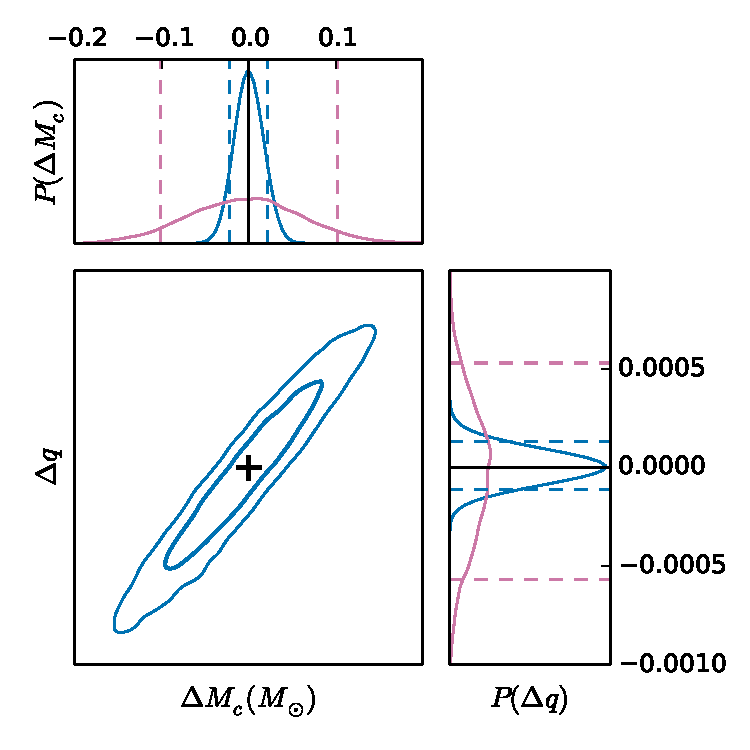
\includegraphics[width=3.4in]{figs/fig1_GR.pdf}
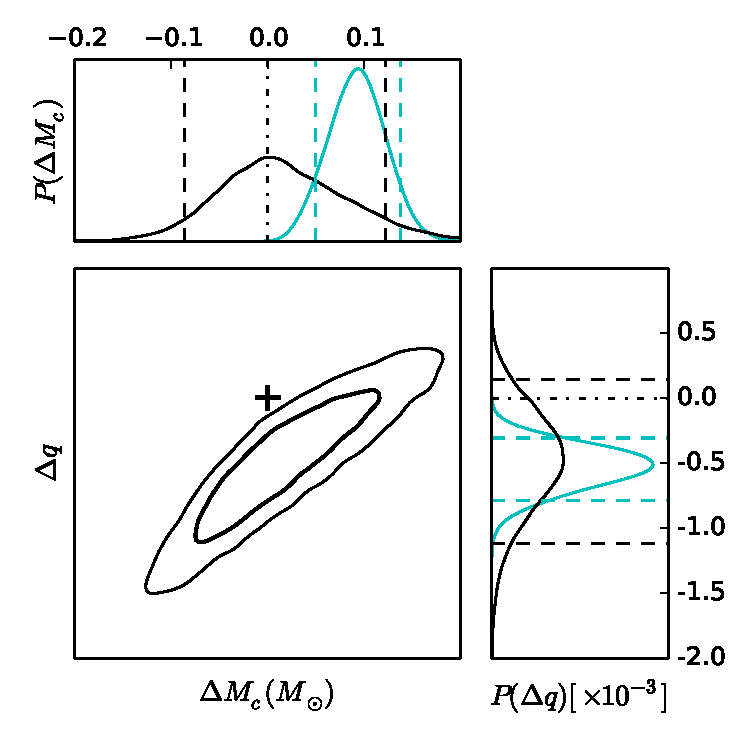
\includegraphics[width=3.4in]{figs/fig1_modGR.pdf}
\caption{The left figure shows 1-D and 2-D posterior distribution of $\Delta \blambda$ for GR waveform.The black 1-D posteriors and 2-D posterior distribution is obtained via varying both $\Delta M_c$ and $\Delta q$.The blue 1-D posterior distribution of $\Delta M_c$  is obtained by fixing $\Delta q$=0.The blue 1-D posterior distribution of $\Delta q$  is obtained by fixing $\Delta M_c$=0.The show agreement with (0,0) for 2-D posteriors and 0 for 1-D posterior distributions.}
\label{fig:contour_plots}
\end{center} \end{figure*}
%%%%%%%%%%%%%%%%%%%%%%%%%%%%%%%%%%%%%%%%%%%%%%%%%%%%%%%%%%%%%%%%%%%%%%%%%%%%%%%%%%%%%%%%%%

An interferometric GW detector observes a linear combination of the two polarizations $h_+(t)$ and $h_\times(t)$ of the GW signal, given by 
\begin{equation}
h(t) = F_+(\theta, \phi, \psi) \, h_+(t-t_0) + F_{\times}(\theta, \phi, \psi)\, {h}_{\times}(t-t_0), 
\label{eq:det_response}
\end{equation}
where $F_+$ and $F_x$ are the antenna pattern functions of the GW detector, $t_0$ is the time of arrival of the signal at the detector, and $(\theta, \phi, \psi)$ define the sky position and polarisation of the GW source respectively. The two GW polarizations $\h := h_+(t) - i \, h_\times(t)$ can be expanded in a basis of spin $-2$ weighted spherical harmonics, as:
\begin{equation}
\h(t; \iota, \phi_0, \blambda) = \sum _{\ell=2}^{\infty} \sum _{m=-\ell}^{\ell} \Ylm (\iota, \phi_0) \, \frac{{\h}_{lm}(t; \blambda)}{d_L}, 
\label{eq:spherical_harmonics}
\end{equation}
where $\Ylm$ are the basis functions of spin $-2$ spherical harmonics, $(\iota, \phi_0)$ define the direction of radiation in the source frame, $d_L$ is  the luminosity distance to the binary, and ${\h}_{lm}(t; \blambda)$ are the spherical harmonic modes of the waveform, which are completely described by the intrinsic parameters $\blambda$ of the system. We assume that the black holes are non-spinning and the binary to be qusi-circular. Hence $\blambda$ consists of only the masses $m_1$ and $m_2$ of the black holes. 

In GR, the set of intrinsic parameters $\blambda$ completely determines the multipolar structure of the waveform ${\h}_{lm}(t)$. Any inconsistency between the different multipoles of the radiation can point to a deviation from GR. In this paper, we propose a test of GR based on the consistency of different multipoles of the gravitational radiation from binary black holes. In order to formulate a consistency test between different multipoles, we rewrite Eq.(\ref{eq:spherical_harmonics}) by splitting the contributions from the dominant $(\ell = 2, m = \pm 2)$ mode of gravitational radiation, and the sub-dominant (higher order) modes 
\begin{eqnarray}
\h(t; \iota, \phi_0, \blambda, \Delta \blambda) & = & \sum_{m = \pm2} Y^{-2}_{2m} (\iota, \phi_0) {\h}_{2m}(t, \blambda)  \nonumber \\ 
 & + & \sum _{\text{H.O.M}} \Ylm (\iota, \phi_0) \h_{lm}(t, \blambda+\Delta \blambda)
\label{eq:test_HM}
\end{eqnarray}
where the subscript H.O.M underneath the summation in the second term on the RHS indicates contribution from just the higher-order multipoles of the gravitational radiation. Note that we allow a possibility of inconsistency between the dominant mode and higher order modes by introducing a deviation $\Delta \blambda$ in the set of intrinsic parameters that describe the higher order modes; in GR,  $\Delta \blambda = 0$. 

The data $d(t)$ contains the observed signal $h(t)$ given in Eq.~(\ref{eq:det_response}) along with noise, which is modeled as a stationary Gaussian random process 
\begin{equation}
d(t) = n(t) + h(t). 
\label{eq:detector_strain}
\end{equation}
For coalescencing binary black hole (BBH) systems in quasi-circular orbits, the observed signal $h(t)$ is described by a set of \emph{intrinsic} parameters $\blambda = \{m_1, m_2\}$ and \emph{extrinsic} parameters  $\btheta := \{t_0, \phi_0, d_L, \theta, \phi, \psi, \iota\}$ in GR. We also introduce a set of parameters $\Delta \blambda$ describing deviations from GR. The combined set of parameters is denoted as $\bxi = \{\blambda, \btheta, \Delta \blambda\}$.  Given data $d$ and assuming a particular model of the waveform as our hypothesis $H$, it is possible to compute the posterior distribution of the set of parameters ${\bxi}$ making use of the Bayes theorem, which states: 
\begin{equation}
P({\bxi} \, | \, d, H) = \frac{P({\bxi} \, | \, H) \, P (d \, | \, {\bxi}, H)}{P(d \, | \, H)}
\label{eq:Bayes_theorem}
\end{equation} 
The first term of the numerator on the RHS, $P({\bxi} \, | \, H)$ is the \emph{prior} distribution of the parameters ${\bxi}$, the second term $P (d \, | \, {\bxi}, H)$ is the \emph{likelihood} function, and the term in the denominator $P(d \, | \, H)$ is a normalisation constant, called the \emph{evidence}. For stationary Gaussian noise with power spectral density $S_n(f)$, the likelihiood can be written as:
\begin{equation}
P (d \, | \, {\bxi}, H) = \text{exp}\Big[ -\frac{1}{2}\int_{f_\mathrm{low}}^{f_\mathrm{high}} \frac{|\tilde{d}(f) - \tilde{h}(f;{\bxi}, H)|^2}{S_n(f)}df\Big]
\end{equation}
where $f_\mathrm{low}$ and $f_\mathrm{high}$ define the sensitivity bandwidth of the detector, while $\tilde{d}(f)$ and $\tilde{h}(f)$ are the Fourier transforms of $d(t)$ and $h(t)$, respectively. 

Using the above definition for the likelihood function, one proceeds to estimate $\bxi$ by stochastically sampling over the entire parameter space of interest. In this work, we use the \textsc{emcee}~\cite{goodman2010ensemble,foreman2013emcee} package, an ensemble Markhov chain Monte-Carlo (MCMC) sampler. \textsc{emcee} uses the underlying property of affine invariance of all Gaussian distributions to sample from highly skewed distributions faster than standard single-particle methods, such as Metropolis-Hastings implementations. A MCMC scheme is a random walk through the parameter space $\bxi$ generating samples of $\bxi$ with a probability density which ultimately converges to the stationary distribution of the Markhov chain, the posterior PDF $P(\bxi|d, H)$, using the equation of detailed balance. An \emph{ensemble} MCMC sampler implements a coordinated random walk of multiple ``walkers" through the parameter space, such that each step of the Markhov chain, or updating the position of any one walker at a paricular time step, is influenced by the positions of the rest of the walkers. The algorithm requires the hand-tuning of a small set of 1-2 parameters, and can be easily parallelised to use multiple CPU cores, giving it major advantages over traditional MCMC algorithms. From the posterior distribution $P(\bxi | d, H)$ of the full parameter set, we construct the posterior distribution $P(\Delta \blambda | d, H)$ of the set of parameters describing deviation from GR prediction, by marginalizing the posterior over all other parameters $\{\blambda, \btheta\}$. If the data is consistent with GR, we expect $P(\Delta \blambda | d, H)$ to be consistent with zero. 

\paragraph{Simulations using GR waveforms:---}
Here we demonstrate this test making use of simulated GW observations from binary black holes where the waveforms are modelled after the GR prediction. We employ the recent waveform model proposed by Mehta \etal~\cite{Mehta:2017zz}, which provide accurate Fourier-domain models of the following spherical harmonic modes $\h_{\ell m}(f)$ of the expected GW from non-spinning binary black holes: $(\ell = 2, m = \pm2)$, $(\ell = 2, m=\pm1)$, $(\ell = 3, m=\pm3)$, $(\ell = 4, m = \pm4)$. GW observations are simulated by combining these signals with stationary Gaussian noise with power spectral density anticipated in Advanced LIGO's ``high-power, zero-detuning'' configuration~\cite{aligo} making use of Eqs.~(\ref{eq:det_response}) and (\ref{eq:det_response}). We employ various choices for the binary's masses as well as orientations. 
 
We perform the test by introducing variations in the higher order modes: The higher-order modes $\hlm(f; \blambda+\Delta\blambda)$ are generated by introducing an extra parameter $\Delta\blambda$ while the quadrupole-modes $\h_{2\pm2}(f; \blambda)$ are generated by using the standard set of parameters $\blambda$ in GR. 

 We have experimented with different choices for the deviation parameter $\Delta\blambda$ --- both by introducing one deviation parameter at a time ($\Delta\blambda = \{\Delta M_c\}$ or $\Delta\blambda = \{\Delta q\}$ where $M_c$ is the chirp mass and $q := m_1/m_2$ is the mass ratio of the binary) and by introducing a combined deviation in two parameters $\Delta \blambda = \{\Delta M_c, \Delta q\}$. We show in Fig.~\ref{fig:contour_plots} (left plot) the results of the tests perforemd by varying either one parameter or two parameters, for the system with total mass $M := m_1 + m_2 = 80M_{\odot}$, mass ratio $q=9$, inclination angle $ {\iota}=60^{\circ} $ producing a signal-to-noise ratin  (SNR)  of 25 (SNR in higher modes is $\sim 10$). It can be seen that the results are consistent with the expected value in GR. As expected, the width of the posteriors are smaller when only one variation is introduced at a time. 

\paragraph{Simulations using modified-GR waveforms:---}

We also investigate the efficacy of our test in detecting deviations from GR. We introduce a deviation from GR in the simulated signals --- a propagation effect predicted by the Chern-Simons (CS) gravity. Under the CS modification to GR, a circularly polarised plane GW, propagating on an Friedmann–Lema\^itre–Robertson–Walker spacetime, would show amplitude birefringence and parity violation~\cite{Yunes:2010yf}. Compared to GR, right circularly polarised waves will be exponentially enhanced or suppressed with respect to left circularly polarized waves, as they propogate. That is, 
% 
\begin{equation}
\h_\mathrm{R,L}^\mathrm{mod} = \h_\mathrm{R,L} \, e^{-i \, \delta\phi_\mathrm{R,L}},
\end{equation}
where $\h_\mathrm{R,L} = (h_+ \pm h_\times)/\sqrt{2}$ are the right/left circularly polarized polarization states predicted by GR and $\delta \phi_{R,L}$ is an additional phase contribution due to the CS correction, given by 
\begin{equation}
\delta \phi_\mathrm{R,L}=i \, \lambda_\mathrm{R,L} \, \pi f z \, \Big(\dot{\theta_0}-\frac{\ddot{\theta_0}}{H_0}\Big).
\end{equation}
Here, $\lambda_\mathrm{R,L}=\pm1$, $f$ is the Fourier frequency measured by the observer, $z$ is the cosmological redshift at source, and ${H_0}$ is the value of the Hubble constant measured by the observer, while $\dot{\theta_0}$ and $\ddot{\theta_0}$ denote the first and second time-derivative of the CS coupling field. Note that the CS correction is purely imaginary which results in amplitude birefringence. Solar system observations of the LAGEOS satellites have allowed us to derive a bound $|\dot{\theta_0}-\frac{\ddot{\theta_0}}{H_0}| < 2000 \mathrm{km}$~\cite{Yunes:2010yf,Smith:2007jm}.

We have constructed such a GR waveform using GR waveforms of $h_+$,$h_{\times}$. Using relations $h_R= \h^\star/\sqrt{2}, ~~ h_L= \h/\sqrt{2}$. One can construct $h_R,h_L$,introduce modification and reconstruct modified $h_+,h_{\times}$. Example of such a modification is shown in Fig.~\ref{fig:mod_gr_waveform} for a system $M = 80M_{\odot}$, $q =9$, $\iota = 90^{\circ}$,solar system constraint at a distance of 200Mpc.The match between GR and modGR waveform is greater than 0.96 for such a departure. If such a modified GR waveform is recovered using GR templates having $h_R(\blambda)$ and $h_L(\blambda+\Delta \blambda)$, one expects the posteriors on $\Delta \blambda$ to not be consistent with zero (right panel of Fig.~\ref{fig:contour_plots}). 
\begin{figure}[h]
	\includegraphics*[width=3.5in]{figs/fig2.pdf}
	\caption{This shows the amplitudes of GR and modified GR for $\delta \phi =i*0.001f$.The system configuration is M=80$M_{\odot}$, q=9, $\iota=90^{\circ}$ at 200Mpc.The match between GR and mod.GR waveform is greater than 0.96 for such a departure.}
\label{fig:mod_gr_waveform}
\end{figure}

\begin{figure}[h]
	\includegraphics*[width=3.5in]{figs/fig3.pdf}
	\caption{This figure shows the 90$\%$ width of $\Delta \blambda/\blambda$ where $\blambda$=M for various configurations of total mass $40M_{\odot}$.The best results of the test can be seen in the systems with high mass ratio.}
\end{figure}

In fig.2 we show the type of systems which give the best results.For a total mass M=40$M_{\odot}$ and total SNR of 25 we show the width of $\Delta M/M$ for various configurations.A system having higher mass ratio will be giving best results in this test.

\paragraph{Conclusions and future work:---} 
Possiblity of observing high mass ratio systems 
Effect of waveform systematics and detector calibration errors 
Combining results from multiple events

%
\bibliographystyle{apsrev-nourl}
\bibliography{TGR_HM}

\end{document}
